\documentclass[twocolumn,8pt]{article}

\topmargin    -10pt % Might need to be set to 0pt 
                      % for some installations

\textheight    610pt
\columnsep      24pt         


\title{GMS Users Manual}

\author{Jo\~{a}o Pedro Jorge\thanks{joajo939@student.liu.se} \and Johannes Rajala\thanks{johra470@student.liu.se}}
\date{30-03-2007}

\usepackage{subfigure}
\usepackage[pdftex]{graphicx}

\begin{document}
\small
\maketitle

\section{Quick Insight}
The application is divided into three main views: MapPlot, Treemap and Parallel Coordinates, and into three secondary views (only Treemaps views).
The application is completely controlled by mouse interaction, and the functionalities are described above.

\section{Views and Interaction}

The following subsections provide the instructions to navigate and interact with the Multi-View functionality of the program. All the views are synchronized in order to give user a coherent view of the data.

\subsection{MapPlot}
This component provides the user with a Geographical overview of the data. There exist 4 types of glyphs \footnote{graphical symbols representing a particular feature of a country}. Those symbols can be selected and unselected just by clicking on the box shown on figure \ref{fig:glyphs}.

\begin{figure}[hbtp]
  \begin{center}
	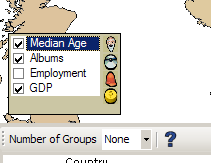
\includegraphics[scale=0.5]{./pics/glyphs.png}
    \caption{Glyph Selection Overview}
    \label{fig:glyphs}
  \end{center}
\end{figure}

Moreover, the other operations that can be done on the map are the following:

\begin{itemize}
\item {\b Panning}: The map can be moved by dragging it while holding the LEFT MOUSE BUTTON.\\

\item {\b Zooming}: The map can be Zoomed Out/In by moving the mouse away/closer from/to the user while holding the RIGHT MOUSE BUTTON.\\

\item {\b Selection of a Country}: A country can be selected by clicking on it with the LEFT MOUSE BUTTON. To select multiple countries, the CONTROL KEY must be hold down while selection is being done with the mouse.\\

\item {\b Tool Tips / Brushing}: To see detailed information regarding a country, just leave the mouse over the desired country and wait a few moments.

\end{itemize}

Finally, the colors can be adjusted by moving the slider on the knob located on the top left corner with the MOUSE LEFT BUTTON.

\subsection{Treemap}

This component provides a view of large amounts of data. To Zoom into a deeper level on a Treemap view, the user just need to click over it with MOUSE LEFT BUTTON. Conversely, to Zoom out, it just need to press the MOUSE RIGHT BUTTON. See Figure
\ref{fig:treemap}.

\begin{figure}[hbtp]
  \begin{center}
	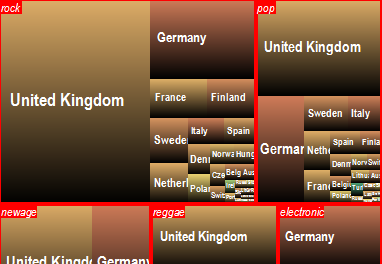
\includegraphics[scale=0.5]{./pics/treemap.png}
    \caption{Treemap Overview}
    \label{fig:treemap}
  \end{center}
\end{figure}

Similarly to the MapPlot, the user can get a detailed information of a Treemap subcomponent by leaving the mouse cursor over it for a few moments.

\subsection{Parallel Coordinates}

This component completes the view of the data and provides an overview of the countries attributes. Each line correspond to a country, and its attribute values are represented by the line intersection with each axis.

The operations that can be done on it are:

\begin{itemize}
\item {\b Select Country}: A country can be selected by moving the mouse over the TableLens (on the left side) or by clicking on the line itself. It works in the same way as the MapPlot.\\
\item {\b Hide Countries}: By moving a slider the user can filter the data given that axis properties.

\end{itemize}

Finally, the user can choose to group the countries using an algorithm that groups them according to similarities (K-Means algorithm). That option is available on the left side of the Toolbar located over the Parallel Coordinates view. See Figure \ref{fig:pcplot}.

\begin{figure}[tp]
  \begin{center}
	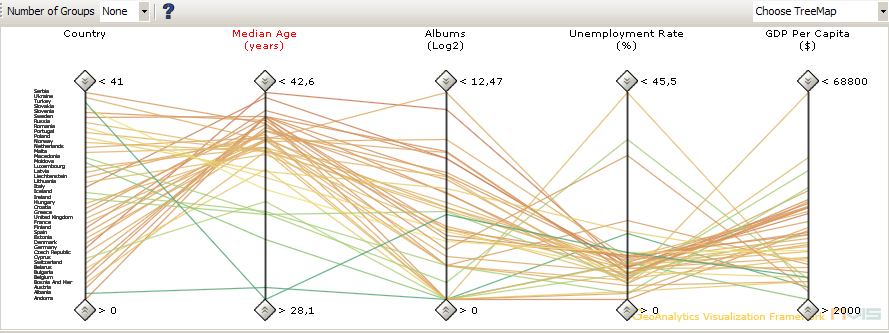
\includegraphics[scale=0.5]{./pics/pcplot.png}
    \caption{Parallel Coordinates Overview}
    \label{fig:pcplot}
  \end{center}
\end{figure}

\subsection{Additional views}

The additional views (can be selected on the combo box on the right side of the toolbar located over the Parallel Coordinates View - see Figure \ref{fig:pcplot}) provide a better insight into the data, and are all Treemap visual structures.


\end{document}
